\documentclass{article}
\usepackage{graphicx}
\usepackage[spanish]{babel}
\graphicspath{ {images/} }

\title{Programación Web y Movil Nativa}
\author{Chamil José Cruz Razeq}

\begin{document}
    \maketitle
    \thispagestyle{empty}
    \newpage
    \tableofcontents
    \newpage

    \section{Introducción}
    Este documento presenta los resultados del ejercicio de evaluación
        de las características de accesibilidad estipulados por la \cite[WCAG]{wcag}
        - Web Content Accesibility Guidelines - presentes en la web y 
        aplicación de Guaguas Global.

    \section{Evaluación Web}
        \begin{figure}[b]
            \includegraphics[scale=0.18]{guaguasglobalwebpage}
            \caption{Guaguas Global página principal}
            \label{fig:mainpage}
        \end{figure}
        \begin{figure}[b]
            \includegraphics[scale=0.18]{guaguasglobalwebpage2}
            \caption{Guaguas Global página principal deslizada}
            \label{fig:mainpage2}
        \end{figure}
        \subsection{Evaluación Inicial}
            Analizando superficialmente la página podemos encontrar varios
             problemas [Figura: \ref{fig:mainpage}] [Figura: \ref{fig:mainpage2}].
            \begin{enumerate}
                \item \textbf{Perceptibilidad:} se establece un menú desplegable
                    el banner principal, dificultando la visibilidad de ambos
                    componentes.
                \item \textbf{Operabilidad:} los menús de navegación y algunos otros
                    elementos se despliegan automaticamente, produciendose en algunas
                    circunstancias despliegues que tapan la información y dificultan
                    interactuar. Adicionalmente, en ciertas circunstancias el
                    despliegue no se produce adecuadamente, provocando que el usuario
                    deba reintentar varias veces acceder a el.
                    Otro aspecto es el banner principal, sobre el que se ubica un menú
                    desplegable que puede presentar dificultades en el acceso de ambos
                    elementos.
                \item \textbf{Comprensibilidad:} se establece el color azul para el
                    \"botón de navegación\" y el color amarillo para el
                    \"botón de mostrar más\" y posteriormente se rompe esta regla
                    visual como podemos observar en la [Figura: \ref{fig:mainpage2}].
                \item \textbf{Robustez:} la página aparenta poseer todas las
                    tecnologías alternativas de navegabilidad, sea por tabulación,
                    narrador...
            \end{enumerate}

        \subsection{Evaluación con Herramienta}
        \begin{figure}
            \centerline{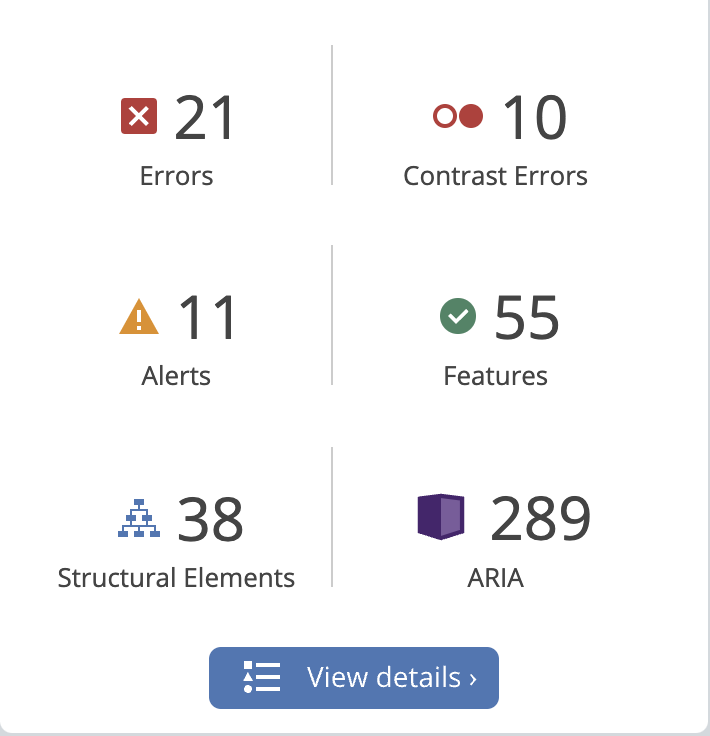
\includegraphics[scale=0.3]{guaguasglobalsum}}
            \caption{Evaluación página Guaguas Global resumida}
            \label{fig:testsum}
        \end{figure}
        \begin{figure}
            \centerline{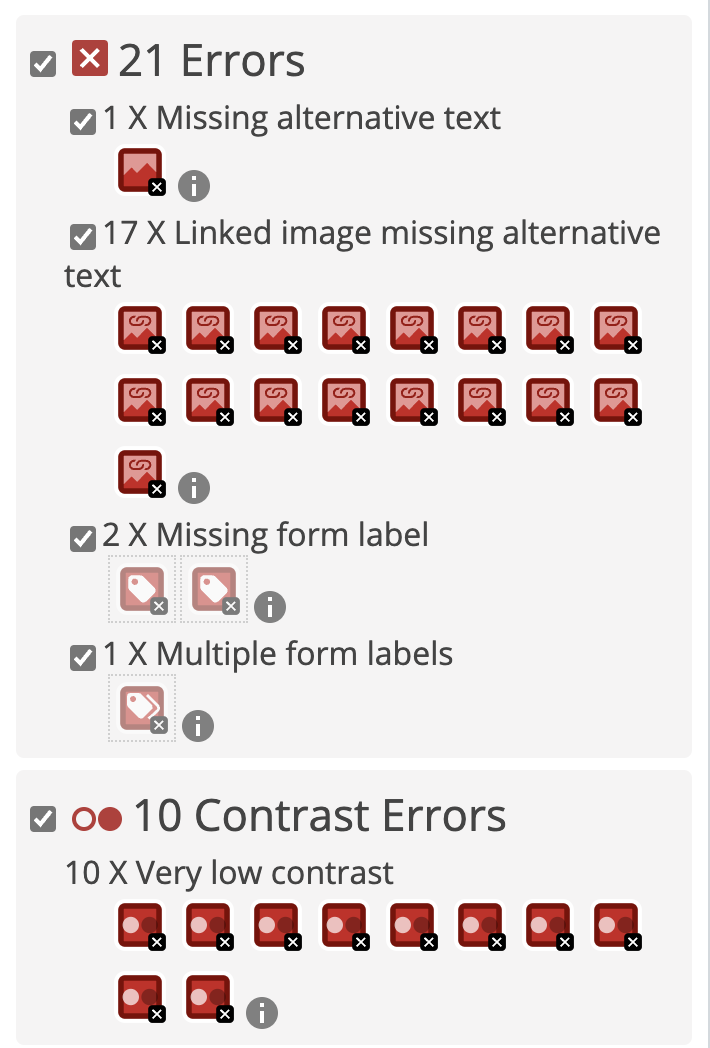
\includegraphics[scale=0.3]{guaguasglobalext}}
            \caption{Evaluación página Guaguas Global extendida}
            \label{fig:testext}
        \end{figure}

        Utilizando la herramiena \cite[WAVE]{wave} hemos obtenidos los resultados
         [Figura: \ref{fig:testsum}] y [Figura: \ref{fig:testext}] que ponen en 
         manifiesto dos claros problemas:
         
         \begin{enumerate}
            \item \textbf{Perceptibilidad:} apreciable en los errores respecto a 
                los errores en cuanto a constraste en algunos elementos.
            \item \textbf{Robustez:} apreciable en los errores respecto a la
                carencia de texto alternativo y \"labels\".
         \end{enumerate}

    \section{Evaluación App}
        \begin{figure}
            \centerline{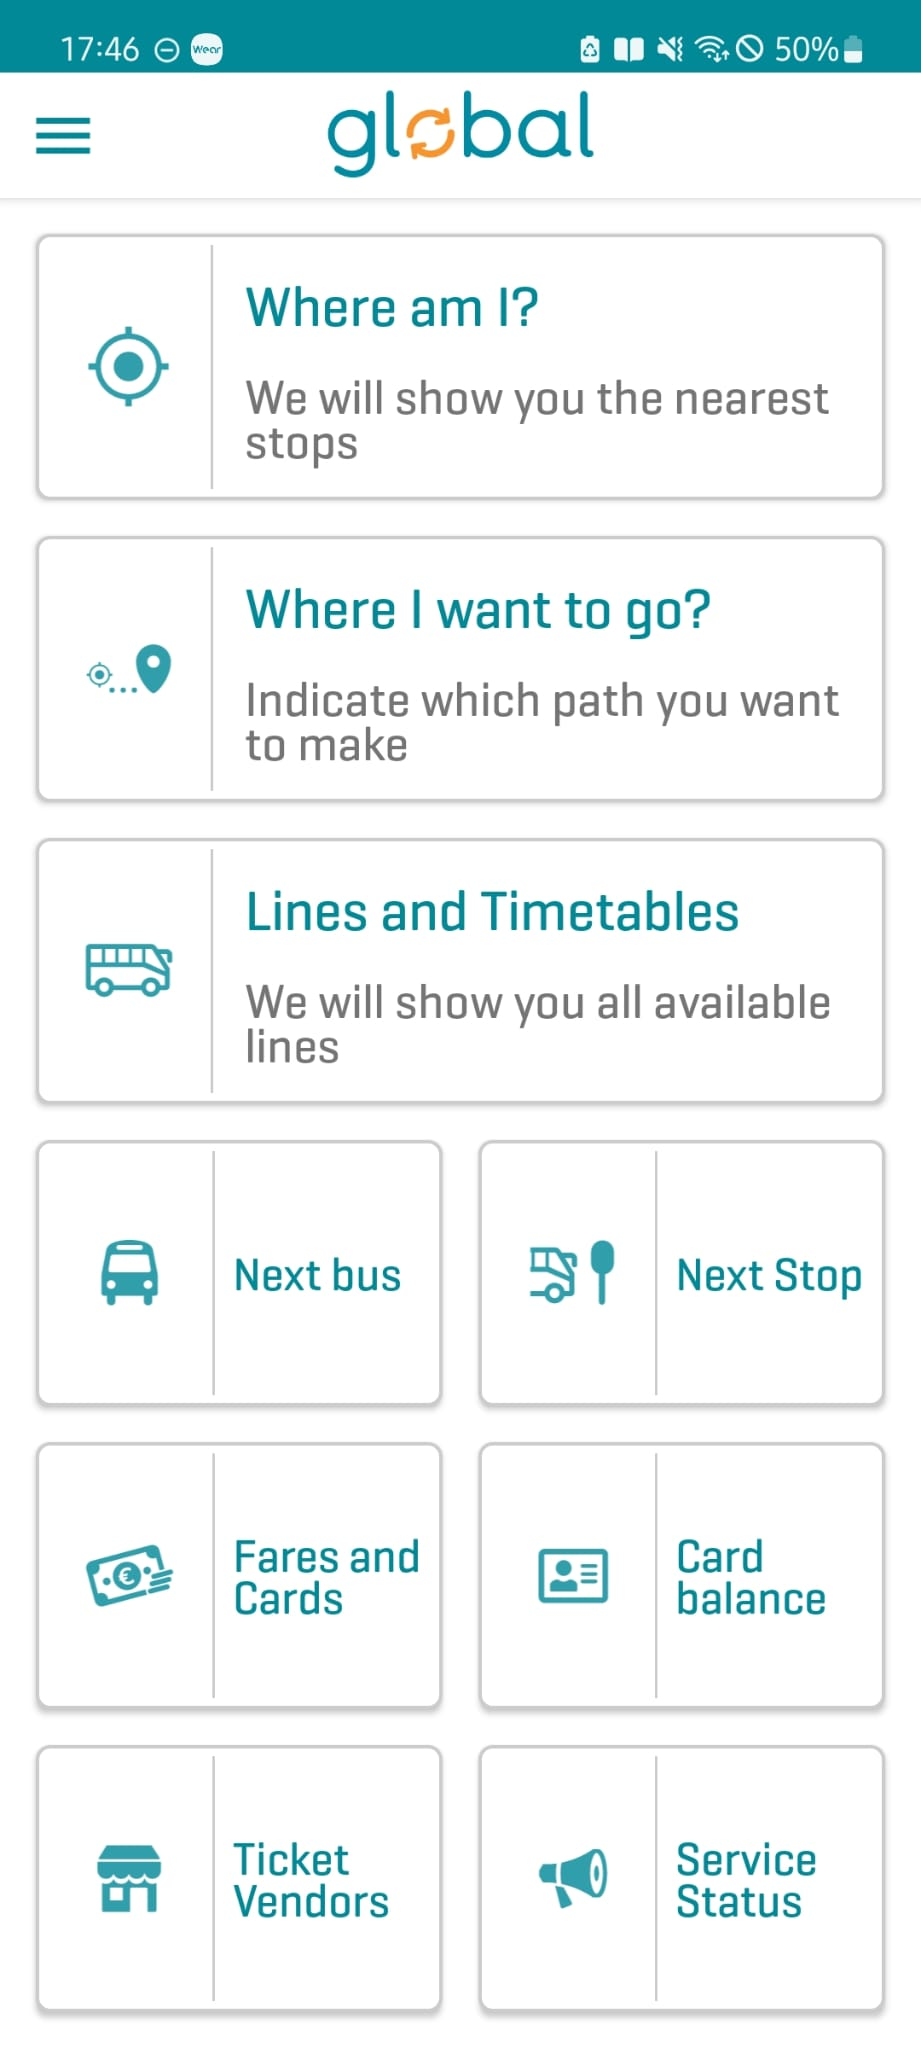
\includegraphics[scale=0.18]{globalapp}}
            \caption{Página principal aplicación de Guaguas Global}
            \label{fig:globalapp}
        \end{figure}

        La aplicación presenta un diseño convencional, con pocos problemas
            apreciables:
        
        \begin{enumerate}
           \item \textbf{Perceptibilidad:} los elementos son grandes y claramente
                delimitados.
            \item \textbf{Operabilidad:} los elementos interactuables están
                suficientemente distanciados y organizados.
           \item \textbf{Comprensibilidad:} los elementos son distinguibles y con
                presencia de iconos acompañados de texto.
           \item \textbf{Robustez:} nada considerable de mención.
        \end{enumerate}

    \section{Conclusión}
    Los resultados anteriores ponen en manifiesto la necesidad de realizar
        tanto evaluaciones superficiales como utilizando herramientas. Ambos
        análisis no son solo retroactivos sino que añaden nuevas consideraciones.
    
    \newpage
    \begin{thebibliography}{9}
        \bibitem{wcag} World Wide Web Consortium (2023) www.w3.org/WAI/standards-guidelines/wcag/es
        \bibitem{wave} Utah State University (2023) wave.webaim.org
        
    \end{thebibliography}

\end{document}
